\documentclass[11pt,a4paper]{article}
\usepackage[utf8]{inputenc}
\usepackage[T1]{fontenc}
\usepackage{amsmath,amsfonts,amssymb}
\usepackage{graphicx}
\usepackage{xcolor}
\usepackage{booktabs}
\usepackage{array}
\usepackage{tabularx}
\usepackage{hyperref}
\usepackage{tikz}
\usetikzlibrary{arrows.meta,positioning,fit,backgrounds,calc}
\usepackage{fancyhdr}
\usepackage{enumitem}
\usepackage{titlesec}
\usepackage{float}
\usepackage{calc}

\definecolor{light-azul}{RGB}{0,102,204}
\usepackage{longtable}
\usepackage{rotating}
% Section formatting
\titleformat{\section}{\Large\bfseries\color{light-azul}}{\thesection}{1em}{}
\titleformat{\subsection}{\large\bfseries\color{light-azul!80}}{\thesubsection}{1em}{}
\titleformat{\subsubsection}{\normalsize\bfseries\color{light-azul!60}}{\thesubsubsection}{1em}{}

% Header/Footer
\pagestyle{fancy}
\fancyhf{}
\renewcommand{\headrulewidth}{0.4pt}

\begin{document}
	
	%=============================================================================
	\section*{Conditionally Selected Platform Configuration\texorpdfstring{\\}{ }and Deployment Baseline}
	%=============================================================================
	
	This document defines the conditionally selected fixed-site spectrum-sensing
	configuration based on the HackRF One R10 and Raspberry Pi~5 for
	\emph{Template~1S: Fixed Single-Node Monitoring}. Named products identify the
	selected baseline implementation; controlled substitutions may be approved
	only when they satisfy the same functional, interface, and acceptance
	requirements.
	
	\textbf{Baseline status: Conditionally selected.} The SDR and compute
	platforms are selected. The complete operational-node baseline remains
	conditional on closure of the sensing-performance criteria, scan plan, RF
	front end, timing interface, secure network configuration, software and
	cybersecurity controls, site installation, controlled bill of materials,
	cost baseline, calibration, and applicable acceptance evidence.
	
	%=============================================================================
	\subsection*{Deployment Requirements}
	%=============================================================================
	
	The approved monitoring plan, \texttt{MP-01}, establishes the operational
	requirements for \emph{Template~1S: Fixed Single-Node Monitoring}. The selected
	hardware and software configuration defined later in this document shall
	satisfy these requirements without expanding the approved scope.
	
	\begin{itemize}[leftmargin=*]
		
		\item \texttt{MP-01-PUR} \emph{Monitoring purpose and intended use.}
		
		The node shall operate continuously at one fixed site and shall perform
		sequential scheduled screening of the approved tuning list. Continuous
		node operation shall not be interpreted as simultaneous or uninterrupted
		observation of every approved band.
		
		The node shall generate screening-grade records for identifying candidate
		events and supporting preliminary technical review. Node records shall not
		independently establish regulatory non-compliance. Formal compliance
		conclusions shall require an approved calibrated measurement and
		evidence-assurance procedure.
		
		\item \texttt{MP-01-JUR} \emph{Jurisdiction and responsible organization.}
		
		The node shall operate within the applicable Colombian
		spectrum-management framework and under the responsibility of the
		organization that owns or operates the monitoring system. No authorization,
		delegation, endorsement, or operational responsibility by the Agencia
		Nacional del Espectro (ANE) shall be inferred unless documented in a
		controlled authorization record.
		
		\item \texttt{MP-01-BND} \emph{Monitored services, bands, and exclusions.}
		
		The authoritative monitoring-band list is defined in
		Appendix~\ref{sec:regulatory-bands}. Exact channels, tuning positions,
		priorities, and effective assignments shall be controlled through
		\texttt{SP-01}.
		
		The 608--614~MHz interval shall remain excluded from the approved DTT scan
		range. The 5350--5470~MHz interval shall remain excluded from the approved
		5-GHz WAS/RLAN scan range unless a separately authorized monitoring
		requirement is established.
		
		\item \texttt{MP-01-SCN} \emph{Scan coverage and observation schedule.}
		
		The controlled scan plan, \texttt{SP-01}, shall define, for every monitored
		service, the tuning positions, channel bandwidths, sample rates, dwell
		times, revisit intervals, retuning and settling allowances, processing
		intervals, maximum scan-cycle duration, exclusion intervals, scan
		priorities, event-interruption behavior, and recovery rules.
		
		\texttt{SP-01} shall also state the minimum event duration expected to be
		observable and the accepted risk of missing short-duration events created
		by sequential scanning. It shall be derived from \texttt{MP-01},
		registered in \texttt{VTM-01}, and verified as feasible before operational
		acquisition begins.
		
		Portable survey operation, simultaneous multiband observation, distributed
		synchronization, direction finding, TDOA, and emitter geolocation are
		outside the approved baseline.
		
		\item \texttt{MP-01-MET} \emph{Required measurands and derived records.}
		
		The node shall generate received-power estimates, center-frequency
		estimates, occupied-bandwidth estimates, spectral-centroid estimates,
		signal-duration records, duty-cycle estimates, channel-occupancy
		statistics, noise-floor estimates, signal-to-noise-ratio estimates, host
		event timestamps, power spectral densities, spectrograms, and event-summary
		records.
		
		\texttt{BA-01-MET} shall define the applicable accuracy, uncertainty,
		detection probability, false-alarm rate, event-detection latency,
		normalization, repeatability, and decision criteria for these outputs.
		
		\item \texttt{MP-01-ACQ} \emph{Acquisition and continuity requirements.}
		
		The acquisition system shall provide complex-IQ data at a sample rate and
		effective bandwidth sufficient for the measurands assigned to each tuning
		position. The selected continuous baseline mode is defined in
		Table~\ref{tab:selected-hardware}.
		
		Alternate or burst modes shall not be used operationally until sustained
		transfer, processing, storage throughput, sample continuity, timing,
		and thermal stability have been verified under \texttt{BA-01-ACQ}.
		
		The platform shall detect, timestamp, and record sample discontinuities,
		receiver overload, clipping, invalid calibration states, storage
		congestion, and processing-queue overflow.
		
		\item \texttt{MP-01-TIM} \emph{Timing, timestamping, and location.}
		
		The 10~MHz reference shall support receiver-frequency stability. The
		GNSS-referenced 1~PPS signal and approved host timing interface shall
		support UTC-referenced host event timestamping.
		
		Event records shall provide a timestamp resolution of 1~ms or better.
		\texttt{BA-01-TIM} shall separately define the maximum timestamp error,
		timestamp origin, processing-latency treatment, holdover behavior,
		discontinuity handling, and reported uncertainty. The baseline shall not
		claim UTC-referenced sample timestamps.
		
		The verified coordinates of the fixed site and the timing-source,
		reference-lock, timestamp-validity, and discontinuity states shall be
		recorded with each applicable observation.
		
		\item \texttt{MP-01-ENV} \emph{Operating environment and installation.}
		
		The node shall operate in dense urban RF conditions containing strong
		broadcast and cellular signals, weak adjacent-channel emissions,
		impulsive interference, multipath propagation, intermittent transmitters,
		near--far conditions, and temperature-dependent receiver variation.
		
		The equipment shall be installed in a protected fixed-site enclosure that
		permits safe inspection, maintenance, and replacement. The complete node
		shall operate within the environmental limits defined in
		\texttt{BA-01-ENV}.
		
		\item \texttt{MP-01-CTX} \emph{Contextual-data requirements.}
		
		Contextual data shall include authorized frequency assignments,
		transmitter-registration records, service-allocation tables, site
		coordinates, antenna records, observation schedules, equipment
		inventories, and applicable technical-limit documents.
		
		Every source shall identify its issuing authority, document identifier,
		revision, effective date, geographic scope, retrieval date, applicability,
		and freshness status.
		
		\item \texttt{MP-01-DAT} \emph{Processing, storage, communication, and
			retention.}
		
		The node shall generate FFT, PSD, spectrogram, occupancy, health, and
		event-summary products locally. Raw IQ shall be retained only following an
		approved event trigger, scheduled validation activity, or authorized
		operator request.
		
		The routine-retention period for metadata, PSD, spectrogram, occupancy,
		health, audit, and event-summary records shall be 90~days. The controlled
		retention policy shall define raw-IQ limits, quotas, overwrite rules,
		storage-reserve thresholds, storage-exhaustion behavior, and investigation
		record retention.
		
		Network transfer shall be restricted to authorized metadata, derived
		products, health records, events, and selected-IQ records.
		
		\item \texttt{MP-01-PWR} \emph{Power and thermal constraints.}
		
		Measured complete-node input power shall remain below 50~W under the
		maximum approved workload. The processing host shall use active cooling,
		and the power and thermal configuration shall satisfy
		\texttt{BA-01-PWR} and \texttt{BA-01-ENV}.
		
		\item \texttt{MP-01-SEC} \emph{Cybersecurity, access control, and audit.}
		
		The node shall implement role-based access control, unique operator
		accounts, key-based remote login, authenticated and encrypted
		administrative and data-transfer connections, controlled software
		updates, versioned configuration changes, restricted service ports,
		backup and restoration, and unauthorized-change detection.
		
		Audit records shall include authentication attempts, administrative
		actions, configuration changes, software updates, service-state changes,
		and data exports.
		
		\item \texttt{MP-01-EVD} \emph{Calibration, provenance, and evidence
			assurance.}
		
		The node shall record equipment identifiers, RF-path configuration,
		antenna and cable identifiers, gain and attenuation states, calibration
		identifiers and validity periods, software and firmware versions,
		sample-continuity indicators, processing history, timing validity, record
		hashes, authorized modifications, and export history.
		
		Template~5 shall apply only to records formally escalated under
		\texttt{MP-01}. Such records shall follow the approved chain-of-custody,
		integrity, uncertainty, retention, access-control, and controlled-export
		requirements.
		
		\item \texttt{MP-01-CST} \emph{Cost and lifecycle basis.}
		
		The USD~1,000--2,000 target shall apply to recurring procurement and
		node-specific integration cost per operational node. It shall include
		controlled hardware, assembly, node-specific commissioning, shipping,
		importation, taxes, initial spares, and contingency. It shall exclude
		separately controlled non-recurring engineering, shared laboratory
		qualification, and five-year lifecycle support.
		
		If the closed recurring per-node cost exceeds USD~2,000, the project shall
		document an approved budget exception, revise only optional capabilities,
		or reopen the platform-selection decision. Mandatory safety, protection,
		acceptance, calibration, cybersecurity, and evidence controls shall not be
		removed solely to satisfy the target.
		
		The five-year lifecycle budget shall separately include calibration,
		replacement storage, software maintenance, spare units, field support,
		site maintenance, backup resources, and component-obsolescence provisions.
		
	\end{itemize}
	
	%=============================================================================
	\subsection*{Phase-0 Controlled-Artifact Registration and Traceability}
	%=============================================================================
	
	\texttt{BA-01} is the controlled \emph{Baseline Acceptance Specification} for
	the conditionally selected platform configuration. It shall be approved,
	placed under configuration control, registered in the Phase-0
	controlled-artifact registry, and anchored in \texttt{VTM-01} before Stage~3
	acceptance testing begins.
	
	The Stage~1 feasibility record, \texttt{FRM-01}, and the Stage~2 comparative
	ranking record, \texttt{CRM-01}, shall be completed and registered in
	\texttt{VTM-01} before Stage~3.
	
	The controlled acceptance sequence shall be:
	
	\[
	\begin{aligned}
		\text{\texttt{MP-01}}
		&\longrightarrow
		\left\{
		\text{\texttt{SP-01}},
		\text{\texttt{BA-01}}
		\right\} \\
		&\longrightarrow
		\text{\texttt{Q3-01}}
		\longrightarrow
		\text{\texttt{T0-*}}
		\longrightarrow
		\text{\texttt{VTM-01}}
		\longrightarrow
		\text{\texttt{EAM-01}}.
	\end{aligned}
	\]
	
	\texttt{Q3-01} shall qualify the laboratory environment used for calibration,
	RF-path characterization, and acceptance testing. \texttt{A5-01} shall apply
	only when Template~5 evidence assurance is invoked for formally escalated
	records.
	
	\paragraph*{BA-01 Minimum Controlled Content}
	
	\texttt{BA-01} shall identify:
	
	\begin{itemize}[leftmargin=*]
		\item the accepted configuration items and revisions;
		\item the applicable \texttt{MP-01} and \texttt{SP-01} identifiers;
		\item the corresponding acceptance criteria and \texttt{T0-*}
		procedures;
		\item the mandatory sensing cases, RF paths, gain and attenuation states,
		acquisition modes, storage configurations, timing states, workloads,
		security states, site conditions, and environmental conditions;
		\item the quantitative thresholds, measurement uncertainty, guard bands,
		and decision rules;
		\item the required calibration, configuration, provenance, integrity,
		cybersecurity, software, site, and audit evidence;
		\item the treatment of invalid, incomplete, repeated, conditional, and
		superseded tests;
		\item the responsible test, review, and approval authorities; and
		\item the evidence package required for the final \texttt{EAM-01}
		decision.
	\end{itemize}
	
	\paragraph*{Required VTM-01 Anchors}
	
	The identifiers in Table~\ref{tab:ba01-vtm-anchors} shall be used as
	controlled \texttt{BA-01} section identifiers and as the corresponding
	\texttt{VTM-01} traceability anchors.
	
	\begin{table}[htbp]
		\centering
		\small
		\renewcommand{\arraystretch}{1.15}
		\begin{tabularx}{\columnwidth}{
				>{\raggedright\arraybackslash}p{3.0cm}
				>{\raggedright\arraybackslash}p{2.5cm}
				>{\raggedright\arraybackslash}X}
			\toprule
			\textbf{Requirement Group} &
			\textbf{BA-01 Anchor} &
			\textbf{Required Verification Evidence} \\
			\midrule
			
			Sensing and measurands &
			\texttt{BA-01-MET} &
			Detection, false-alarm, latency, power, frequency, bandwidth,
			noise-floor, SNR, occupancy, PSD, repeatability, and uncertainty tests \\
			
			Acquisition and continuity &
			\texttt{BA-01-ACQ} &
			Sample-continuity, sustained-throughput, scan-cycle, dwell,
			retuning, queue, and maximum-workload tests \\
			
			RF-path performance &
			\texttt{BA-01-RF} &
			Insertion-loss, rejection, isolation, return-loss, overload,
			sensitivity, gain-state, attenuation-state, switching, and calibration
			tests \\
			
			Timing and timestamping &
			\texttt{BA-01-TIM} &
			Frequency-reference, event-timestamp resolution and error,
			reference-lock, holdover, reacquisition, and continuity tests \\
			
			Storage and records &
			\texttt{BA-01-STR} &
			Throughput, retention, quota, congestion, interrupted-write,
			recovery, and record-integrity tests \\
			
			Power and fault recovery &
			\texttt{BA-01-PWR} &
			Load, regulation, ripple, startup, interruption, branch-protection,
			isolation, and recovery tests \\
			
			Environment and enclosure &
			\texttt{BA-01-ENV} &
			Thermal, humidity, cooling-failure, enclosure, grounding, bonding,
			surge-protection, and environmental tests \\
			
			Software and services &
			\texttt{BA-01-SW} &
			Configuration reproducibility, processing correctness, bounded-queue,
			service-startup, restart, watchdog, degraded-state, and recovery tests \\
			
			Cybersecurity and audit &
			\texttt{BA-01-SEC} &
			Authentication, authorization, encryption, restricted-service,
			update, backup, restoration, audit, export-control, and
			unauthorized-change tests \\
			
			Site commissioning &
			\texttt{BA-01-SIT} &
			Installed antenna, cable, grounding, bonding, surge-protection,
			timing, network, enclosure, cooling, access-control, and site tests \\
			
			Evidence assurance &
			\texttt{BA-01-EVD} &
			Provenance, calibration validity, integrity, chain-of-custody,
			retention, access-control, and controlled-export checks, including
			\texttt{A5-01} where Template~5 is invoked \\
			
			\bottomrule
		\end{tabularx}
		\caption{Minimum VTM-01 anchors for BA-01-controlled acceptance}
		\label{tab:ba01-vtm-anchors}
	\end{table}
	
	Each anchor shall be dispositioned in \texttt{EAM-01} as
	\emph{Accepted}, \emph{Conditionally Accepted}, or \emph{Rejected}, supported
	by the applicable controlled evidence.
	
	Any change to \texttt{BA-01}, \texttt{SP-01}, or the selected configuration
	after test execution begins shall require a documented impact assessment,
	versioned approval, and identification of all tests and evidence that must be
	repeated, revalidated, or superseded.
	
	%=============================================================================
	\subsection*{Baseline Hardware Infrastructure}
	%=============================================================================
	
	The controlled hardware baseline shall comprise the configuration in
	Table~\ref{tab:selected-hardware}. Device capabilities that exceed the approved
	operational configuration shall not be interpreted as accepted operating
	modes.
	
	\begin{table}[htbp]
		\centering
		\small
		\renewcommand{\arraystretch}{1.2}
		\begin{tabularx}{\columnwidth}{
				>{\raggedright\arraybackslash}p{2.8cm}
				>{\raggedright\arraybackslash}p{4.1cm}
				>{\raggedright\arraybackslash}X}
			\toprule
			\textbf{Controlled Item} &
			\textbf{Baseline Selection} &
			\textbf{Controlled Implication} \\
			\midrule
			
			SDR platform &
			HackRF One R10; 1~MHz--6~GHz device range; 8-bit ADC;
			USB~2.0; half-duplex; 10~MHz CLKIN &
			Approved for receive-only monitoring. Every RF path and gain state
			shall be characterized under \texttt{BA-01-RF}. USB continuity and
			overload behavior shall be verified under \texttt{BA-01-ACQ} \\
			
			Continuous acquisition &
			Single-channel complex IQ at 10~Msps using signed 8-bit interleaved
			samples &
			This is the approved continuous mode. Higher sample rates are
			alternate or burst modes and require separate
			\texttt{BA-01-ACQ} verification \\
			
			Compute platform &
			Raspberry Pi~5 with 8~GB RAM and active cooling &
			Shall support bounded buffering, FFT/PSD processing, detection,
			metadata generation, storage, and network operation under the
			maximum approved simultaneous workload \\
			
			Local storage &
			At least 2~TB of approved NVMe-class storage connected through an
			approved interface &
			Sustained throughput, congestion handling, retention, recovery, and
			record integrity shall satisfy \texttt{BA-01-STR} \\
			
			Timing reference &
			GNSS-disciplined 10~MHz frequency reference and 1~PPS timing signal &
			Frequency stability, reference-lock status, timestamp error, and
			timing continuity shall satisfy \texttt{BA-01-TIM} \\
			
			Network interface &
			Gigabit Ethernet through a protected enclosure entry &
			Supports authenticated and encrypted transfer of authorized metadata,
			derived records, events, health records, and selected IQ \\
			
			Control interfaces &
			Raspberry Pi~5 GPIO, SPI, and I\textsuperscript{2}C interfaces &
			Supports antenna and preselector switching, attenuation and LNA
			control, timing/status inputs, and subsystem health monitoring \\
			
			Power architecture &
			Regulated complete-node source rated for at least 40~W continuous
			output, including a dedicated 5~V/5~A Raspberry Pi rail and
			independently protected auxiliary outputs &
			Startup current, transient response, voltage regulation, branch
			protection, interruption recovery, and maximum-load operation shall
			satisfy \texttt{BA-01-PWR} \\
			
			Installation and environmental protection &
			Lockable fixed-site enclosure with active cooling, temperature
			monitoring, protected RF, power, timing, and Ethernet entries,
			grounding, bonding, surge protection, strain relief,
			corrosion-resistant mounting, and service access &
			Thermal performance, environmental protection, grounding, bonding,
			surge-current routing, cable support, and safe maintenance access
			shall satisfy \texttt{BA-01-ENV} \\
			
			\bottomrule
		\end{tabularx}
		\caption{Controlled baseline hardware configuration and acceptance
			implications}
		\label{tab:selected-hardware}
		
	\end{table}
	
	\paragraph*{Configuration Control and Acceptance}
	
	The controlled procurement bill of materials shall identify the manufacturer,
	model, part number, revision, electrical and environmental ratings, connector
	or interface type, mounting method, and operating-temperature range for every
	baseline component.
	
	The Raspberry Pi~5 implementation shall use bounded processing queues,
	sample-continuity monitoring, controlled buffering, and health monitoring.
	Acceptance shall be performed under simultaneous acquisition, processing,
	storage, network, timing, cooling, and RF-control operation.
	
	No hardware item, interface, gain state, acquisition mode, or environmental
	configuration shall be released for operational use until the applicable
	\texttt{BA-01-ACQ}, \texttt{BA-01-RF}, \texttt{BA-01-TIM},
	\texttt{BA-01-STR}, \texttt{BA-01-PWR}, \texttt{BA-01-ENV},
	\texttt{BA-01-SW}, \texttt{BA-01-SEC}, and \texttt{BA-01-SIT} criteria have
	been satisfied.
	
	%=============================================================================
	\subsection*{Selected RF Front End}
	%=============================================================================
	
	The controlled RF chain shall be:
	
	\[
	\begin{aligned}
		\text{Antenna}
		&\rightarrow
		\text{Primary antenna-line surge protection}
		\rightarrow
		\text{Antenna selector} \\
		&\rightarrow
		\text{Secondary limiter/DC block}
		\rightarrow
		\text{Preselector}
		\rightarrow
		\text{LNA/Bypass} \\
		&\rightarrow
		\text{Attenuator/Bypass}
		\rightarrow
		\text{HackRF One}.
	\end{aligned}
	\]
	
	The RF front end shall protect the receiver, limit out-of-band loading, and
	provide reproducible RF-path, gain, and attenuation states. Every selected
	state shall be recorded with the corresponding monitoring record.
	
	\paragraph*{Antenna Subsystem}
	
	\begin{table}[htbp]
		\centering
		\small
		\renewcommand{\arraystretch}{1.2}
		\begin{tabularx}{\columnwidth}{
				>{\raggedright\arraybackslash}p{3.0cm}
				>{\raggedright\arraybackslash}p{2.8cm}
				>{\raggedright\arraybackslash}X}
			\toprule
			\textbf{Antenna} &
			\textbf{Frequency Range} &
			\textbf{Controlled Application} \\
			\midrule
			
			BicoLOG 5070 &
			70--700~MHz &
			Approved VHF, lower-UHF, land-mobile, and DTT monitoring paths \\
			
			HyperLOG 7060 &
			700~MHz--6~GHz &
			Approved 700--960~MHz, 2.4-GHz, and 5-GHz monitoring paths \\
			
			\bottomrule
		\end{tabularx}
		\caption{Controlled antenna configuration}
		\label{tab:antennas}
	\end{table}
	
	Each rooftop antenna feed shall include approved primary antenna-line surge
	protection before the antenna selector unless a controlled installation study
	demonstrates equivalent protection. An absorptive SPDT antenna selector or
	equivalent shall connect exactly one protected antenna feed to the downstream
	RF chain. Its insertion loss, isolation, switching time, power handling,
	fail-safe state, and environmental rating shall be verified under
	\texttt{BA-01-RF} and \texttt{BA-01-SIT}.
	
	\paragraph*{Protection and Preselector Assembly}
	
	The antenna-selector output shall pass through the approved secondary limiter
	and DC block before entering the preselector. The preselector shall use paired
	absorptive SP8T input and output selectors operated synchronously. The eight
	selector positions shall comprise seven filtered paths and one protected
	bypass path.
	
	\begin{table}[htbp]
		\centering
		\small
		\renewcommand{\arraystretch}{1.2}
		\begin{tabularx}{\columnwidth}{
				>{\raggedright\arraybackslash}p{3.0cm}
				>{\raggedright\arraybackslash}p{4.2cm}
				>{\raggedright\arraybackslash}X}
			\toprule
			\textbf{Selector Position} &
			\textbf{Controlled RF Path} &
			\textbf{Required Function} \\
			\midrule
			
			1 &
			88--108~MHz FM-bandpass assembly &
			Support FM monitoring. Any notch substate shall be separately
			controlled, calibrated, and recorded \\
			
			2 &
			108--137~MHz aeronautical bandpass assembly &
			Support the approved aeronautical radionavigation and communications
			monitoring scope \\
			
			3 &
			406--470~MHz land-mobile bandpass assembly &
			Support the approved private land-mobile monitoring range \\
			
			4 &
			Two-port dual-passband DTT assembly for
			470--608~MHz and 614--698~MHz &
			Support DVB-T2 channels 14--36 and 38--51 while rejecting
			608--614~MHz \\
			
			5 &
			700--960~MHz UHF/cellular bandpass assembly &
			Support the approved 700-, 800-, and 900-MHz monitoring ranges \\
			
			6 &
			2400--2483.5~MHz ISM/WAS/RLAN bandpass assembly &
			Support the approved 2.4-GHz monitoring range \\
			
			7 &
			Two-port dual-passband 5-GHz WAS/RLAN assembly for
			5150--5350~MHz and 5470--5850~MHz &
			Support the approved 5-GHz subbands while rejecting
			5350--5470~MHz \\
			
			8 &
			Protected 50~$\Omega$ bypass path &
			Support approved maintenance, characterization, and bypass operation
			without removing receiver-input protection \\
			
			\bottomrule
		\end{tabularx}
		\caption{Controlled preselector positions}
		\label{tab:preselector}
	\end{table}
	
	The DTT and 5-GHz dual-passband assemblies are conditionally selected pending
	RF-feasibility closure. Each shall present one controlled two-port path between
	the paired SP8T selectors. Before configuration freeze, the project shall
	identify a realizable circuit or commercial implementation and shall close its
	passband, ripple, return-loss, rejection, isolation, power-handling,
	temperature-response, physical-integration, and procurement requirements.
	Successful prototype verification under \texttt{BA-01-RF} is mandatory.
	
	The selector fail-safe state shall disconnect the HackRF input or select the
	protected bypass path. The Raspberry Pi~5 shall control the antenna and
	preselector selectors through an approved GPIO, SPI, or
	I\textsuperscript{2}C interface.
	
	\paragraph*{Gain and Attenuation Assembly}
	
	The selected preselector output shall pass through an approved LNA/bypass
	stage and an approved attenuator/bypass stage. \texttt{BA-01-RF} shall define
	the permitted state for every preselector position.
	
	\begin{table}[htbp]
		\centering
		\small
		\renewcommand{\arraystretch}{1.2}
		\begin{tabularx}{\columnwidth}{
				>{\raggedright\arraybackslash}p{3.2cm}
				>{\raggedright\arraybackslash}p{2.8cm}
				>{\raggedright\arraybackslash}X}
			\toprule
			\textbf{Component or State} &
			\textbf{Validated Range} &
			\textbf{Controlled Function} \\
			\midrule
			
			Passive LNA bypass &
			All approved bands &
			Default state where the accepted sensitivity criterion is satisfied
			without external amplification \\
			
			Band-specific VHF LNA &
			88--137~MHz &
			Conditional weak-signal amplification for approved VHF paths \\
			
			Band-specific lower-UHF LNA &
			406--500~MHz &
			Conditional amplification for the land-mobile path and lower portion
			of the DTT path \\
			
			ZX60-33LN-S+ or equivalent &
			0.5--4~GHz &
			Conditional amplification only within its validated range \\
			
			Band-specific 5-GHz LNA &
			Approved 5-GHz subbands &
			Conditional weak-signal amplification for the 5-GHz path \\
			
			Attenuator bypass &
			All approved bands &
			Approved state where external attenuation is unnecessary and overload
			criteria remain satisfied \\
			
			ZX76-31R75PP-S+ or equivalent &
			0.1--4~GHz &
			Programmable attenuation for approved sub-4-GHz paths \\
			
			Band-specific 5-GHz attenuator &
			Approved 5-GHz subbands &
			Conditional attenuation where required by the accepted 5-GHz
			overload-control strategy \\
			
			\bottomrule
		\end{tabularx}
		\caption{Controlled gain, bypass, and attenuation states}
		\label{tab:lna}
	\end{table}
	
	Every LNA, bypass device, and attenuator shall be identified in the controlled
	bill of materials and validated for frequency response, gain or attenuation
	accuracy, noise figure where applicable, compression, overload behavior,
	isolation, switching transients, settling time, temperature response, and
	calibration stability.
	
	\paragraph*{Gain-Control Strategy}
	
	Gain-state thresholds, hysteresis, and minimum state-hold times shall be
	defined and verified under \texttt{BA-01-RF}. The implementation shall:
	
	\begin{enumerate}
		\item monitor FFT peak level, broadband RMS level, clipping, and overload
		indicators;
		\item disable the LNA, select LNA bypass, increase attenuation, or select
		attenuator bypass according to the approved per-path state table;
		\item enable amplification or reduce attenuation only when the resulting
		state satisfies the validated sensitivity and overload criteria;
		\item prevent rapid or unstable gain-state switching; and
		\item record the antenna, selector position, filter assembly, LNA state,
		attenuator state, receiver-gain state, and calibration revision with every
		applicable record.
	\end{enumerate}
	
	\paragraph*{RF Acceptance and Configuration Control}
	
	The controlled bill of materials shall identify the antenna-line protection,
	antenna selector, secondary limiter, DC block, both SP8T selectors, every
	filter assembly, LNA, bypass device, attenuator, connector, cable, enclosure,
	and control interface.
	
	Acceptance under \texttt{BA-01-RF} shall characterize every approved antenna,
	filter, gain, attenuation, and bypass combination for insertion loss, ripple,
	usable bandwidth, stopband rejection, inactive-path isolation, return loss,
	sensitivity, overload behavior, switching transients, settling time,
	temperature response, and calibration correction.
	
	%=============================================================================
	\subsection*{Timing and Synchronization}
	%=============================================================================
	
	The fixed node shall use a GNSS-disciplined timing subsystem to provide:
	
	\begin{itemize}[leftmargin=*]
		\item a 10~MHz frequency reference for HackRF receiver-frequency
		stability; and
		\item a 1~PPS signal for UTC-referenced host timing and event
		timestamping.
	\end{itemize}
	
	The timing subsystem shall satisfy the frequency-offset, event-timestamp
	resolution, maximum event-timestamp error, reference-lock, continuity,
	startup-readiness, holdover, and loss-of-reference criteria defined in
	\texttt{BA-01-TIM}. The baseline shall not claim UTC-referenced sample
	timestamps.
	
	\begin{table}[htbp]
		\centering
		\small
		\renewcommand{\arraystretch}{1.2}
		\begin{tabularx}{\columnwidth}{
				>{\raggedright\arraybackslash}p{1.6cm}
				>{\raggedright\arraybackslash}p{2.4cm}
				>{\raggedright\arraybackslash}p{3.4cm}
				>{\raggedright\arraybackslash}X}
			\toprule
			\textbf{Signal} &
			\textbf{Source} &
			\textbf{Destination} &
			\textbf{Controlled Function} \\
			\midrule
			
			
			10~MHz &
			GPSDO reference output &
			HackRF CLKIN &
			Discipline receiver-frequency generation and support residual
			frequency-offset correction \\
			
			1~PPS &
			GPSDO PPS output &
			Raspberry Pi~5 PPS-capable kernel interface or approved
			hardware-timestamping interface &
			Discipline UTC-referenced host time and validate the resolution, origin,
			maximum error, uncertainty, and continuity of host-assigned event timestamps \\
			
			Timing status &
			GPSDO status interface &
			Raspberry Pi~5 monitoring service &
			Record GNSS lock, oscillator discipline, holdover state,
			reference loss, reacquisition, and timing validity \\
			
			\bottomrule
		\end{tabularx}
		\caption{Controlled timing-reference distribution}
		\label{tab:timing}
		
		
	\end{table}
	
	A generic userspace GPIO timestamp shall not be used as evidence of compliance
	with the timestamp-error criterion. Any GPIO-based 1~PPS implementation shall
	use an approved kernel PPS interface or hardware-assisted capture method and
	shall be characterized under the maximum approved processing workload.
	
	The timing service shall record:
	
	\begin{itemize}[leftmargin=*]
		\item the active timing source and GPSDO identifier;
		\item GNSS-lock, discipline, and holdover status;
		\item 10~MHz reference availability;
		\item 1~PPS continuity and detected discontinuities;
		\item UTC synchronization status and estimated timestamp error;
		\item timing calibration and correction identifiers; and
		\item the validity state associated with each applicable observation.
	\end{itemize}
	
	Following loss of GNSS lock, 10~MHz reference, or 1~PPS continuity, affected
	records shall be marked with the applicable degraded or invalid timing state.
	Operational timestamp validity shall not be restored until the reacquisition
	and stability criteria defined in \texttt{BA-01-TIM} have been satisfied.
	
	The HackRF trigger interface may be used for repeatable local laboratory tests
	or controlled triggered acquisition. It shall not be represented as evidence
	of UTC sample alignment, phase coherence, inter-node synchronization, or
	sample-synchronous operation unless those capabilities are separately
	implemented and validated.
	
	Distributed synchronization, TDOA, phase-coherent processing, and sample-level
	alignment across nodes remain outside the approved
	\emph{Template~1S: Fixed Single-Node Monitoring} baseline.
	
	\begin{figure}[H]
	\centering
	
	\resizebox{0.92\textwidth}{!}{%
		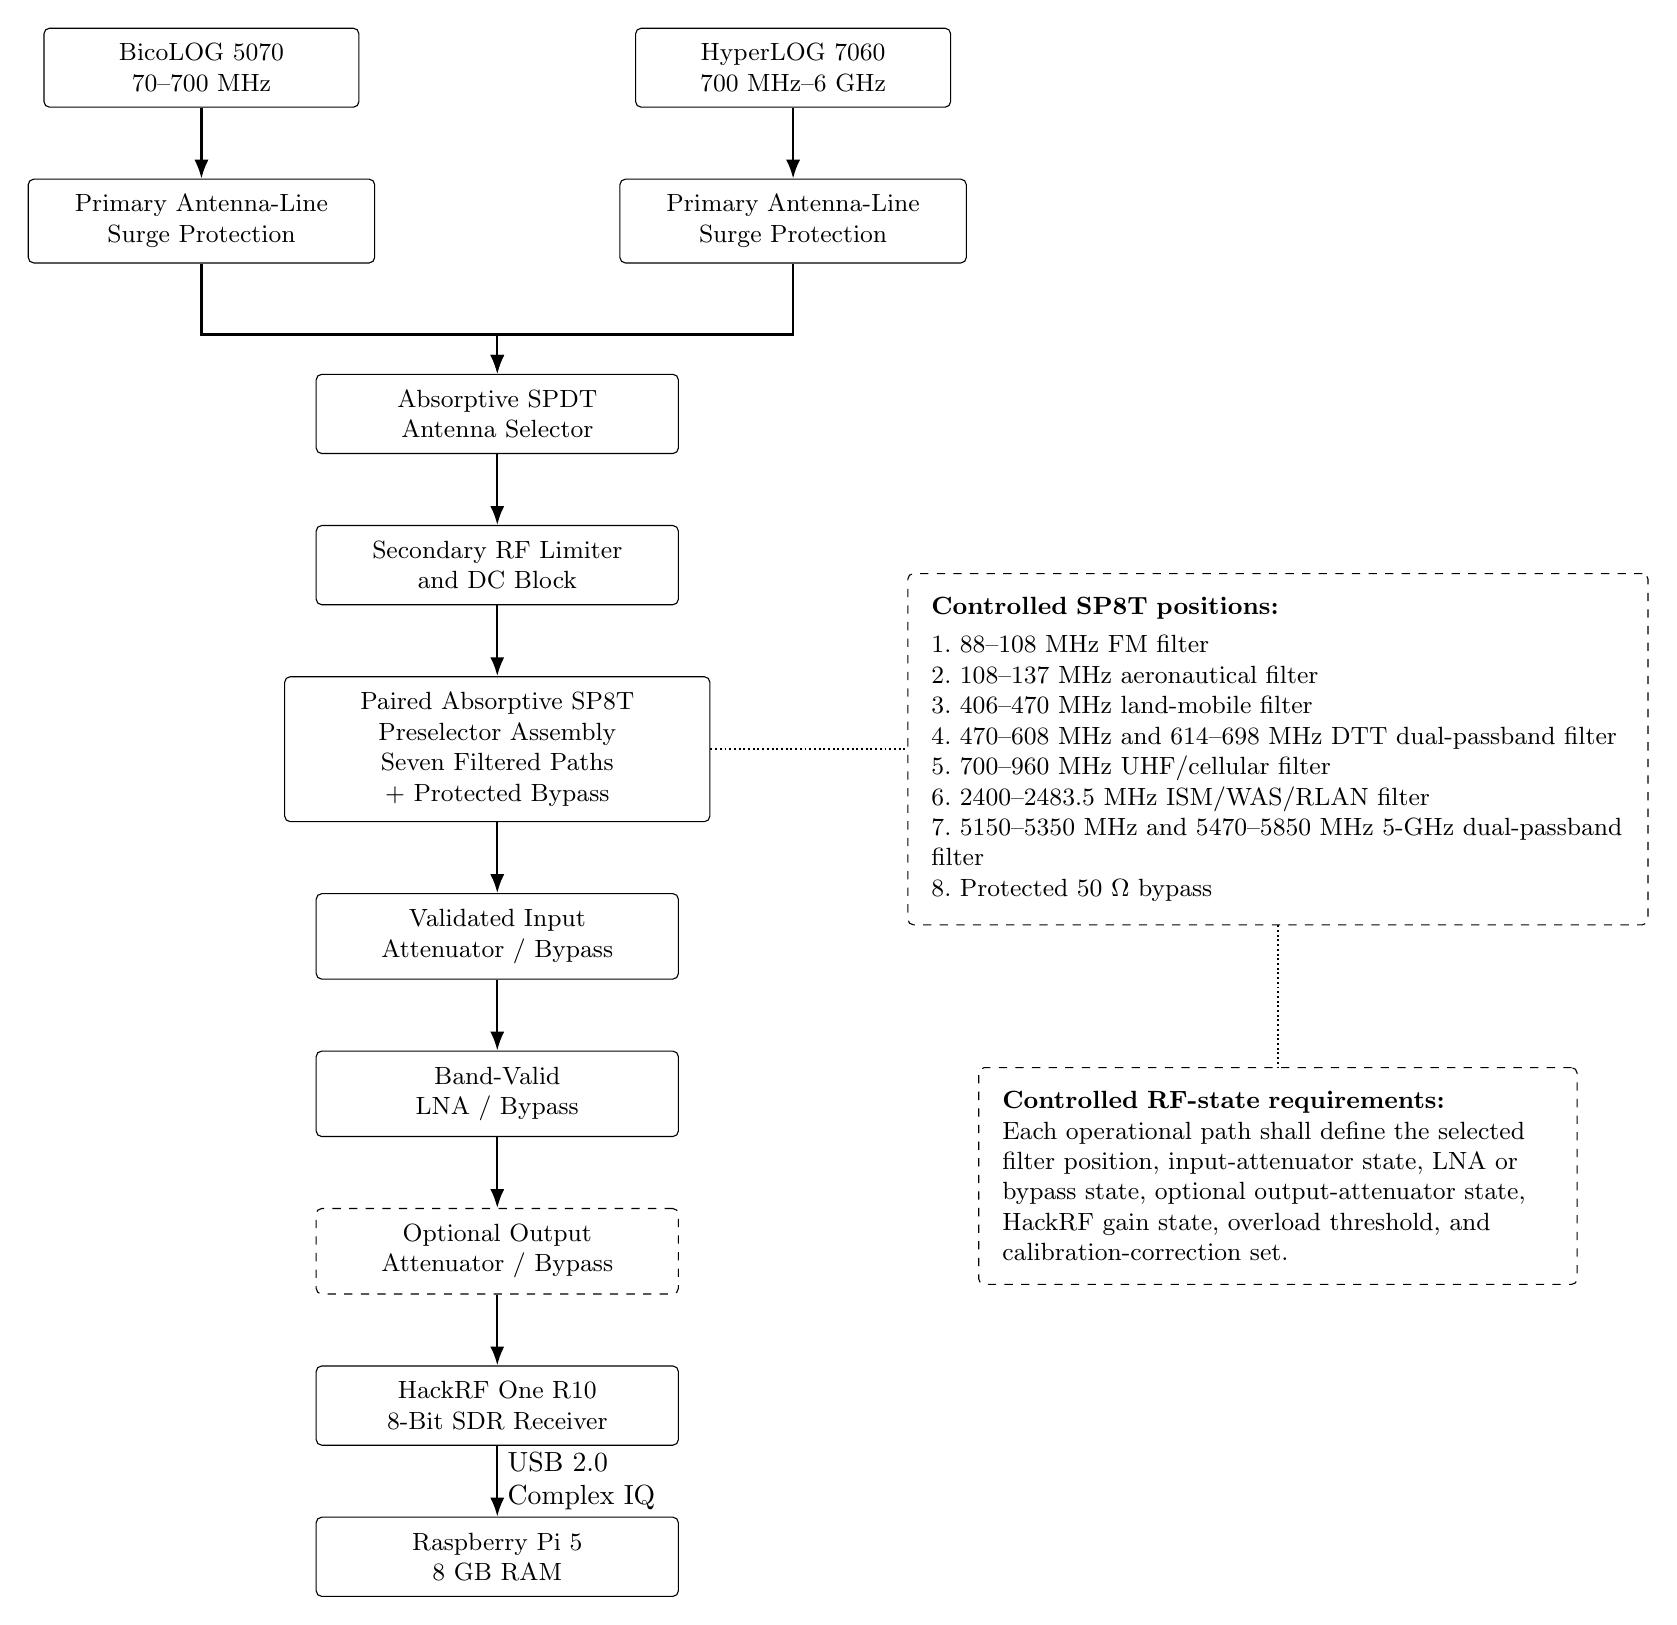
\begin{tikzpicture}[
			>=Latex,
			node distance=9mm and 18mm,
			signal/.style={
				-{Latex[length=2.4mm]},
				line width=0.85pt
			},
			association/.style={
				densely dotted,
				line width=0.7pt
			},
			block/.style={
				draw,
				rounded corners=2pt,
				align=center,
				minimum height=10mm,
				text width=42mm,
				inner sep=2mm,
				font=\small
			},
			antenna/.style={
				draw,
				rounded corners=2pt,
				align=center,
				minimum height=10mm,
				text width=36mm,
				inner sep=2mm,
				font=\small
			},
			protection/.style={
				draw,
				rounded corners=2pt,
				align=center,
				minimum height=10mm,
				text width=40mm,
				inner sep=2mm,
				font=\small
			},
			preselector/.style={
				draw,
				rounded corners=2pt,
				align=center,
				minimum height=13mm,
				text width=50mm,
				inner sep=2mm,
				font=\small
			},
			pathlist/.style={
				draw,
				dashed,
				rounded corners=2pt,
				align=left,
				text width=88mm,
				inner sep=3mm,
				font=\small
			},
			optional/.style={
				draw,
				dashed,
				rounded corners=2pt,
				align=center,
				minimum height=10mm,
				text width=42mm,
				inner sep=2mm,
				font=\small
			}
			]
			
			%=====================================================================
			% Antenna subsystem
			%=====================================================================
			
			\node[antenna] (ant1)
			{BicoLOG 5070\\70--700~MHz};
			
			\node[antenna, right=35mm of ant1] (ant2)
			{HyperLOG 7060\\700~MHz--6~GHz};
			
			\node[protection, below=of ant1] (surge1)
			{Primary Antenna-Line\\Surge Protection};
			
			\node[protection, below=of ant2] (surge2)
			{Primary Antenna-Line\\Surge Protection};
			
			\coordinate (surge-mid)
			at ($(surge1.south)!0.5!(surge2.south)$);
			
			\node[block, below=14mm of surge-mid] (antsw)
			{Absorptive SPDT\\Antenna Selector};
			
			\draw[signal] (ant1) -- (surge1);
			\draw[signal] (ant2) -- (surge2);
			
			\draw[signal]
			(surge1.south)
			|- ($(antsw.north)+(0,5mm)$)
			-- (antsw.north);
			
			\draw[signal]
			(surge2.south)
			|- ($(antsw.north)+(0,5mm)$)
			-- (antsw.north);
			
			%=====================================================================
			% Core controlled RF path
			%=====================================================================
			
			\node[block, below=of antsw] (limiter)
			{Secondary RF Limiter\\and DC Block};
			
			\node[preselector, below=of limiter] (preselector)
			{Paired Absorptive SP8T\\Preselector Assembly\\
				Seven Filtered Paths + Protected Bypass};
			
			\node[block, below=of preselector] (inputatt)
			{Validated Input\\Attenuator / Bypass};
			
			\node[block, below=of inputatt] (lna)
			{Band-Valid\\LNA / Bypass};
			
			\node[optional, below=of lna] (outputatt)
			{Optional Output\\Attenuator / Bypass};
			
			\node[block, below=of outputatt] (hackrf)
			{HackRF One R10\\8-Bit SDR Receiver};
			
			\node[block, below=of hackrf] (pi)
			{Raspberry Pi~5\\8~GB RAM};
			
			\draw[signal] (antsw) -- (limiter);
			\draw[signal] (limiter) -- (preselector);
			\draw[signal] (preselector) -- (inputatt);
			\draw[signal] (inputatt) -- (lna);
			\draw[signal] (lna) -- (outputatt);
			\draw[signal] (outputatt) -- (hackrf);
			
			\draw[signal]
			(hackrf)
			--
			node[right,align=left]
			{USB~2.0\\Complex IQ}
			(pi);
			
			%=====================================================================
			% Controlled preselector positions
			%=====================================================================
			
			\node[
			pathlist,
			right=25mm of preselector
			] (paths)
			{
				\textbf{Controlled SP8T positions:}\\[1mm]
				1.\ 88--108~MHz FM filter\\
				2.\ 108--137~MHz aeronautical filter\\
				3.\ 406--470~MHz land-mobile filter\\
				4.\ 470--608~MHz and 614--698~MHz
				DTT dual-passband filter\\
				5.\ 700--960~MHz UHF/cellular filter\\
				6.\ 2400--2483.5~MHz ISM/WAS/RLAN filter\\
				7.\ 5150--5350~MHz and 5470--5850~MHz
				5-GHz dual-passband filter\\
				8.\ Protected 50~$\Omega$ bypass
			};
			
			\draw[association]
			(preselector.east)
			--
			(paths.west);
			
			%=====================================================================
			% Functional annotations
			%=====================================================================
			
			\node[
			pathlist,
			text width=70mm,
			below=18mm of paths
			] (states)
			{
				\textbf{Controlled RF-state requirements:}\\
				Each operational path shall define the selected filter position,
				input-attenuator state, LNA or bypass state, optional
				output-attenuator state, HackRF gain state, overload threshold,
				and calibration-correction set.
			};
			
			\draw[association]
			(paths.south)
			--
			(states.north);
			
		\end{tikzpicture}%
	}
	
	\caption{Controlled RF architecture for the fixed-site
		70~MHz--6~GHz spectrum-sensing node.
		Operational monitoring is restricted to the controlled preselector
		bands and scan plan.}
	\label{fig:controlled-rf-architecture}
	
\end{figure}
	
	%=============================================================================
	\subsection*{Selected Software Architecture}
	%=============================================================================
	
	The software architecture shall separate hardware access, streaming
	acquisition, signal processing, record management, assurance, security, and
	network transport. Hardware-specific settings and calibration data shall remain
	isolated from higher-level detection, record-generation, and export logic.
	
	All deployed software packages, dependencies, configurations, processing
	parameters, and calibration files shall be identified by version and integrity
	hash in the controlled software configuration.
	
	\begin{table}[htbp]
		\centering
		\small
		\renewcommand{\arraystretch}{1.2}
		\begin{tabularx}{\columnwidth}{
				>{\raggedright\arraybackslash}p{2.7cm}
				>{\raggedright\arraybackslash}p{3.8cm}
				>{\raggedright\arraybackslash}X}
			\toprule
			\textbf{Layer} &
			\textbf{Controlled Component} &
			\textbf{Controlled Responsibility} \\
			\midrule
			
			SDR access &
			libhackrf and SoapySDR-HackRF &
			Device discovery, initialization, tuning, sample-rate selection,
			sample-format control, receiver-gain control, clock-source selection,
			and isolation of hardware-specific arguments \\
			
			Streaming acquisition &
			GNU Radio streaming runtime &
			Bounded buffering, sample-continuity monitoring, discontinuity
			detection, DC-offset conditioning, timestamp association, queue-state
			monitoring, and controlled backpressure or record dropping \\
			
			Signal processing and detection &
			GNU Radio, Python, NumPy, and SciPy &
			FFT and PSD generation, averaging, noise-floor estimation, occupancy
			calculation, threshold detection, event formation, and approved
			derived-measurand generation \\
			
			Record and metadata management &
			SigMF records and controlled event, health, and audit schemas &
			Associate each record with the antenna, RF path, gain and attenuation
			states, receiver settings, timing state, calibration revision,
			software version, processing parameters, and quality indicators \\
			
			Local storage and retention &
			Controlled record manager on approved NVMe storage &
			Atomic record creation, storage-quota enforcement, retention,
			overwrite control, congestion detection, recovery, and selected-IQ
			capture management \\
			
			Integrity and export assurance &
			Hash-manifest and audit-record service &
			Generate integrity hashes, record processing and modification history,
			authorize exports, and preserve the identity of every exported
			evidence package \\
			
			Network transport &
			ZeroMQ over an approved authenticated and encrypted TCP transport &
			Transfer only approved metadata, events, health records, derived
			products, and explicitly authorized IQ records; authentication and
			encryption shall be provided by the approved transport-security
			configuration \\
			
			Service and health management &
			systemd, watchdog, and health-monitoring services &
			Controlled startup, dependency ordering, supervision, fault
			detection, restart limits, degraded-state handling, and shutdown \\
			
			Host security and configuration &
			Linux access controls, key-based SSH, restricted services, and
			versioned configuration &
			Role-based administration, update control, configuration provenance,
			backup and restoration, unauthorized-change detection, and
			administrative auditing \\
			
			\bottomrule
		\end{tabularx}
		\caption{Controlled software architecture}
		\label{tab:software}
		
	\end{table}
	
	\paragraph*{Controlled Processing Flow}
	
	The approved processing sequence shall be:
	
	\[
	\begin{aligned}
		\text{SDR acquisition}
		&\rightarrow
		\text{IQ conditioning and continuity monitoring} \\
		&\rightarrow
		\text{FFT/PSD and derived-measurand generation} \\
		&\rightarrow
		\text{detection and event formation} \\
		&\rightarrow
		\text{metadata, health, and integrity records} \\
		&\rightarrow
		\text{local retention and authorized publication}.
	\end{aligned}
	\]
	
	Event-triggered IQ recording shall operate as a controlled branch from the
	event-formation stage. Failure of that branch shall not silently interrupt the
	generation of continuity, health, or fault records.
	
	\paragraph*{Mandatory Runtime Controls}
	
	The implementation shall:
	
	\begin{itemize}[leftmargin=*]
		\item use bounded queues and explicitly defined queue-overflow behavior;
		\item detect and record sample loss, clipping, invalid timestamps,
		reference-clock loss, processing overruns, storage congestion, and service
		failures;
		\item use only the approved FFT window, transform size, overlap, averaging,
		normalization, and detection-threshold configuration;
		\item apply detection thresholds to calibrated or consistently normalized
		PSD estimates;
		\item associate every output with its source capture, processing
		configuration, RF-path state, timing state, calibration revision, and
		software revision;
		\item prevent raw-IQ publication unless the active controlled
		configuration explicitly authorizes the transfer;
		\item generate integrity hashes and auditable records for configuration
		changes, processing, modification, retention, and export actions;
		\item preserve fault and quality states across service restarts where
		required to interpret affected records; and
		\item enter a controlled degraded or failed state when mandatory
		acquisition, timing, storage, metadata, or integrity services are
		unavailable.
	\end{itemize}
	
	\paragraph*{Software Acceptance and Change Control}
	
	Acceptance shall verify simultaneous acquisition, processing, storage,
	network, timing, and RF-control operation under the maximum approved workload.
	Testing shall include sample continuity, bounded-queue behavior, service
	restart, storage congestion, interrupted writes, configuration restoration,
	record integrity, unauthorized export prevention, and fault recovery.
	
	Alternative software components, processing parameters, metadata schemas,
	transport mechanisms, or deployment configurations shall require a controlled
	configuration change, traceability update, and revalidation under the
	applicable \texttt{BA-01-ACQ}, \texttt{BA-01-STR}, and
	\texttt{BA-01-SW}, \texttt{BA-01-SEC}, and \texttt{BA-01-EVD} criteria.
	
	%=============================================================================
	\subsection*{Power and Thermal Design}
	%=============================================================================
	
	Table~\ref{tab:power} provides the provisional power budget used to size the
	controlled power architecture defined in
	Table~\ref{tab:selected-hardware}. The values are planning estimates and shall
	be replaced or confirmed using the approved component specifications and
	measured maximum-load results.
	
	\begin{table}[htbp]
		\centering
		\small
		\renewcommand{\arraystretch}{1.2}
		\begin{tabularx}{\columnwidth}{
				>{\raggedright\arraybackslash}X
				>{\centering\arraybackslash}p{2.6cm}
				>{\centering\arraybackslash}p{2.6cm}}
			\toprule
			\textbf{Load} &
			\textbf{Nominal Planning Load} &
			\textbf{Maximum Planning Load} \\
			\midrule
			
			
			Raspberry Pi~5 with active cooling &
			7.0~W &
			15.0~W \\
			
			HackRF One R10 &
			2.0~W &
			3.0~W \\
			
			LNA/bypass assembly &
			0.5~W &
			0.8~W \\
			
			Programmable attenuation assembly &
			0.1~W &
			0.2~W \\
			
			Antenna selector, paired SP8T selectors, and control electronics &
			0.1~W &
			0.5~W \\
			
			GPSDO and timing-interface hardware &
			1.0~W &
			2.0~W \\
			
			NVMe storage device and interface &
			1.5~W &
			5.0~W \\
			\midrule
			
			\textbf{Estimated DC-load subtotal} &
			\textbf{12.2~W} &
			\textbf{26.5~W} \\
			
			Conversion and distribution allowance$^{*}$ &
			1.8~W &
			4.0~W \\
			\midrule
			
			\textbf{Provisional complete-node design load} &
			\textbf{14.0~W} &
			\textbf{30.5~W} \\
			
			\bottomrule
		\end{tabularx}
		
		\vspace{1mm}
		
		\begin{minipage}{0.96\columnwidth}
			\footnotesize
			$^{*}$The conversion and distribution allowance provisionally represents
			DC--DC conversion losses, wiring losses, protection-device losses, and
			unallocated low-power control loads. Acceptance shall use measured
			values from the final controlled configuration.
		\end{minipage}
		
		\caption{Provisional complete-node power budget}
		\label{tab:power}
		
	\end{table}
	
	\paragraph*{Power-System Sizing}
	
	The controlled baseline shall use a regulated complete-node power source rated
	for at least 40~W of continuous DC output. Relative to the provisional
	30.5~W maximum design load, this provides approximately 9.5~W of unallocated
	DC-output capacity for startup current, load transients, component variation,
	and controlled configuration changes.
	
	The 40~W rating is a minimum power-source output capability. The
	\texttt{MP-01} limit of 50~W applies to measured complete-node input-power
	consumption under the maximum approved workload, including power-conversion
	losses.
	
	Each powered branch shall have documented nominal voltage, maximum current,
	conductor rating, connector rating, protection device, disconnect method, and
	fault-isolation behavior. The Raspberry Pi~5 shall use its dedicated regulated
	5~V/5~A rail; RF, storage, timing, switching, and cooling loads shall use
	appropriately regulated and independently protected auxiliary branches.
	
	\paragraph*{Thermal Design}
	
	The enclosure and cooling configuration shall be sized for the heat generated
	at the maximum approved electrical load and the highest ambient temperature
	defined in \texttt{BA-01-ENV}. Temperature monitoring shall cover, at minimum,
	the Raspberry Pi~5 processor, NVMe device, HackRF, GPSDO, RF front end, and
	enclosure air or representative internal thermal reference.
	
	The controlled configuration shall define:
	
	\begin{itemize}[leftmargin=*]
		\item maximum allowable component and enclosure temperatures;
		\item temperature-warning and controlled-shutdown thresholds;
		\item cooling-failure detection and response;
		\item airflow or conductive heat-transfer requirements;
		\item startup restrictions following overtemperature shutdown; and
		\item the temperature and power telemetry retained in health records.
	\end{itemize}
	
	\paragraph*{Electrical and Thermal Acceptance}
	
	Acceptance under \texttt{BA-01-PWR} and \texttt{BA-01-ENV} shall verify:
	
	\begin{itemize}[leftmargin=*]
		\item steady-state and transient power consumption under the maximum
		simultaneous acquisition, processing, storage, network, timing, cooling,
		and RF-control workload;
		\item startup and inrush-current behavior;
		\item voltage regulation and ripple at every powered branch;
		\item branch protection, short-circuit isolation, and recovery;
		\item controlled recovery following input-power interruption;
		\item maximum internal temperatures at the approved environmental limits;
		\item cooling degradation or failure behavior; and
		\item compliance with the 40~W minimum source capacity and the 50~W
		complete-node input-power limit.
	\end{itemize}
	
	The final controlled power budget shall use measured maximum values from the
	accepted hardware configuration. Any change that increases the maximum
	electrical or thermal load shall require an updated budget and revalidation
	under the applicable \texttt{BA-01-PWR} and \texttt{BA-01-ENV} criteria.
	
	%=============================================================================
	\subsection*{Cost Baseline}
	%=============================================================================
	
	The cost baseline shall distinguish recurring per-node cost, provisional
	allowances, configuration-dependent items, non-recurring engineering, and
	five-year lifecycle cost. The USD~1,000--2,000 target defined in
	\texttt{MP-01-CST} applies only to recurring procurement and node-specific
	integration cost per operational node.
	
	\paragraph*{Current Priced-Item Register}
	
	The values in Table~\ref{tab:bom} are preliminary planning values. They are not
	supplier-validated costs unless supported by a dated quotation in the
	controlled procurement register.
	

\begin{longtable}{
        >{\raggedright\arraybackslash}p{5.8cm}
        >{\centering\arraybackslash}p{1.2cm}
        >{\centering\arraybackslash}p{2.0cm}
        >{\raggedright\arraybackslash}p{3.4cm}}
    \caption{Current preliminary cost register}
    \label{tab:bom}\\
    \toprule
    \textbf{Item} &
    \textbf{Qty.} &
    \textbf{Planning Value (USD)} &
    \textbf{Cost Classification} \\
    \midrule
    \endfirsthead

    \multicolumn{4}{c}{\tablename\ \thetable\ -- continued} \\
    \toprule
    \textbf{Item} &
    \textbf{Qty.} &
    \textbf{Planning Value (USD)} &
    \textbf{Cost Classification} \\
    \midrule
    \endhead

    \midrule
    \multicolumn{4}{r}{Continued on next page} \\
    \endfoot

    \bottomrule
    \endlastfoot

    HackRF One Pro &
    1 &
    400 &
    Mandatory; preliminary value \\

    Raspberry Pi~5 with 8~GB RAM &
    1 &
    175 &
    Mandatory; preliminary value \\

    Raspberry Pi~5 active cooler &
    1 &
    5 &
    Mandatory; preliminary value \\

    Proxicast ANT-127-002 &
    1 &
    144 &
    Mandatory; converted from supplier price \\

    Diamond D130NJ Super Discone &
    1 &
    129 &
    Mandatory \\

    Paired SP8T selectors and control hardware &
    1 set &
    15 &
    Mandatory; selector set only; part numbers not closed \\

    GPSDO/reference-clock module &
    1 &
    185 &
    Mandatory; excludes antenna, cables, and PPS interface \\

    ZX76-31R75PP-S+ or equivalent &
    1 &
    222 &
    Mandatory for approved programmable-attenuation paths within its
    validated range \\

    RF-filter prototype allowance &
    1 &
    615 &
    Provisional allowance; shall be replaced by separately closed costs
    for all seven filter assemblies and the bypass implementation \\

    Enclosure and mounting allowance &
    1 &
    120 &
    Provisional allowance; shall be replaced by the complete accepted
    enclosure and mounting cost \\

    Cables and connectors allowance &
    1 &
    50 &
    Provisional allowance; shall be replaced by the production
    interconnection cost \\

    ZX60-33LN-S+ or equivalent &
    1 &
    227 &
    Configuration-dependent; included in the planning budget \\

    \midrule

    \textit{Equipment subtotal} &
    &
    2,287 &
    Sum of all listed items (mandatory, provisional, and configuration-dependent) \\

    \textit{Unforeseen expenses (10\% contingency)} &
    &
    229 &
    Budget reserve for integration, shipping, fabrication, and procurement uncertainties \\

    \textbf{Total project budget} &
    &
    \textbf{2,516} &
    Equipment subtotal (2,287 USD) + contingency (229 USD) \\
\end{longtable}



	
	\paragraph*{Mandatory Unpriced Configuration Items}
	
	The controlled procurement bill of materials shall identify, price, and close:
	
	\begin{itemize}[leftmargin=*]
		\item at least 2~TB of approved NVMe storage and its interface;
		\item the protected antenna selector and its control hardware;
		\item primary antenna-line protection for each antenna feed;
		\item the secondary limiter and DC block;
		\item all seven filter assemblies, the protected bypass path, internal
		combining networks, shielding, connectors, and assembly hardware;
		\item any selected VHF, lower-UHF, general-purpose, or 5-GHz LNA;
		\item any selected 5-GHz attenuator;
		\item the GPSDO antenna, timing cables, PPS interface, and mounting
		hardware;
		\item the complete regulated power source, conversion modules,
		distribution hardware, branch protection, wiring, and disconnects;
		\item the final fixed-site enclosure, mounting plate, cooling,
		temperature sensors, protected entries, grounding, bonding, and
		surge-protection hardware;
		\item production RF cables, adapters, connectors, Ethernet hardware, and
		mechanical supports;
		\item shipping, importation, taxes, procurement fees, and supplier
		minimum-order effects;
		\item node-specific assembly, installation, and commissioning; and
		\item initial operational spares and the approved contingency.
	\end{itemize}
	
	A provisional allowance shall be removed when the corresponding controlled
	item is priced. The closed cost shall replace the allowance and shall not be
	added to it.
	
	\paragraph*{Recurring Per-Node Cost}
	
	The recurring cost of one accepted operational node shall be calculated as:
	
	\[
	C_{\mathrm{node}}
	=
	C_{\mathrm{hardware}}
	+
	C_{\mathrm{conditional}}
	+
	C_{\mathrm{integration}}
	+
	C_{\mathrm{procurement}}
	+
	C_{\mathrm{spares}}
	+
	C_{\mathrm{contingency}}.
	\]
	
	The controlled cost register shall define the quantity, supplier, quotation
	date, currency basis, exchange-rate basis where applicable, and inclusion or
	exclusion of taxes for every cost entry.
	
	\paragraph*{Non-Recurring and First-Article Costs}
	
	The non-recurring cost register shall separately record RF-filter and
	enclosure design, prototype fabrication, corrective redesign,
	calibration-method development, software integration, cybersecurity
	hardening, acceptance-procedure development, laboratory fixtures, reference
	equipment, qualification testing, and controlled documentation.
	
	The first-article cost shall be reported as:
	
	\[
	C_{\mathrm{first}}
	=
	C_{\mathrm{node}}
	+
	C_{\mathrm{NRE}}.
	\]
	
	If non-recurring costs are distributed across multiple nodes, the allocation
	method and production quantity shall be documented.
	
	\paragraph*{Cost-Control Decision}
	
	Budget compliance shall be evaluated only after every mandatory item has a
	controlled quantity and cost, every provisional allowance has been replaced,
	every selected conditional item has been included, and procurement,
	integration, spares, and contingency have been closed.
	
	If \(C_{\mathrm{node}}>2{,}000~\text{USD}\), the project shall approve a budget
	exception, revise only optional capabilities without violating
	\texttt{MP-01} or \texttt{BA-01}, or reopen the platform-selection decision.
	
	Mandatory RF protection, timing, storage, power, enclosure, thermal,
	grounding, calibration, cybersecurity, sensing-performance, or acceptance
	requirements shall not be removed solely to satisfy the target.
	
	\paragraph*{Lifecycle Cost}
	
	The five-year lifecycle budget shall be maintained separately from
	\(C_{\mathrm{node}}\) and \(C_{\mathrm{first}}\). It shall include scheduled
	calibration, replacement storage, component failures, spare units, software
	maintenance, field support, site maintenance, backup resources, and
	component-obsolescence mitigation.
	
	%=============================================================================
	\subsection*{Key Limitations and Controls}
	%=============================================================================
	
	Table~\ref{tab:limitations} identifies residual platform limitations that
	remain after implementation of the selected controls. A mitigation shall not
	be treated as closure until the applicable \texttt{BA-01} criterion has been
	verified and the evidence has been registered in \texttt{VTM-01}.
	
	\begin{longtable}{
			>{\raggedright\arraybackslash}p{3.0cm}
			>{\raggedright\arraybackslash}p{5.7cm}
			>{\raggedright\arraybackslash}p{5.0cm}}
		\caption{Residual platform limitations and mandatory controls}
		\label{tab:limitations}\\
		\toprule
		\textbf{Residual Limitation} &
		\textbf{Operational Consequence} &
		\textbf{Mandatory Control and Acceptance Anchor} \\
		\midrule
		\endfirsthead
		
		\multicolumn{3}{c}{\tablename\ \thetable\ -- continued} \\
		\toprule
		\textbf{Residual Limitation} &
		\textbf{Operational Consequence} &
		\textbf{Mandatory Control and Acceptance Anchor} \\
		\midrule
		\endhead
		
		\midrule
		\multicolumn{3}{r}{Continued on next page} \\
		\endfoot
		
		\bottomrule
		\endlastfoot
		
		8-bit quantization and limited instantaneous dynamic range &
		Strong signals may cause overload, clipping, desensitization, or
		masking of weaker signals &
		Preselection, validated gain and attenuation states, overload
		detection, and dynamic-range testing under \texttt{BA-01-RF} and
		\texttt{BA-01-MET} \\
		
		Single-tuner sequential scanning &
		Separated bands cannot be observed simultaneously; scan gaps may miss
		short events &
		Controlled dwell, revisit, scan-cycle, event-priority, interruption,
		recovery, and missed-event criteria under \texttt{SP-01},
		\texttt{BA-01-ACQ}, and \texttt{BA-01-MET} \\
		
		USB~2.0 acquisition interface &
		Sustained-transfer margin is limited at higher sample rates and
		simultaneous host workloads &
		Maintain the validated continuous mode and verify sample continuity,
		queue behavior, and alternate modes under \texttt{BA-01-ACQ} \\
		
		RF-path-dependent sensitivity and insertion loss &
		Detection performance and calibration vary by antenna, filter, LNA,
		attenuation, and bypass state &
		Characterize every approved RF-path combination under
		\texttt{BA-01-RF} and verify sensing outputs under
		\texttt{BA-01-MET} \\
		
		Conditional active-component coverage &
		General-purpose gain and attenuation components do not cover every
		approved band &
		Define an accepted LNA/bypass and attenuator/bypass state for every
		filter path under \texttt{BA-01-RF} \\
		
		Unclosed composite filter assemblies &
		DTT and 5-GHz path feasibility, loss, rejection, integration, and cost
		remain uncertain &
		Complete prototype, RF, environmental, integration, and cost closure
		before configuration freeze \\
		
		Host, storage, and processing contention &
		Simultaneous DSP, recording, networking, and storage may cause queue
		overflow, incomplete records, latency, or sample loss &
		Bounded queues, explicit overflow behavior, storage-reserve controls,
		health monitoring, and maximum-workload testing under
		\texttt{BA-01-ACQ}, \texttt{BA-01-STR}, and \texttt{BA-01-SW} \\
		
		Host-assigned event timing &
		Valid UTC event timestamps do not establish UTC-aligned sample indices,
		phase coherence, or inter-node synchronization &
		Verify timestamp origin, resolution, maximum error, uncertainty,
		holdover, and continuity under \texttt{BA-01-TIM} \\
		
		Single-node observation &
		The baseline cannot independently provide TDOA, direction finding,
		geolocation, or cross-node confirmation &
		Restrict outputs to the approved fixed single-node scope; require a
		separate profile and acceptance specification for distributed
		capabilities \\
		
		Environmental and thermal dependence &
		Temperature, humidity, cooling degradation, and enclosure conditions
		may affect stability, storage, timing, and calibration &
		Verify maximum-load operation and environmental limits under
		\texttt{BA-01-PWR}, \texttt{BA-01-ENV}, and \texttt{BA-01-SIT} \\
		
		Screening-grade evidentiary status &
		Node records alone are insufficient for an independent regulatory
		non-compliance finding &
		Preserve calibration, provenance, timing, quality, and integrity
		metadata and apply Template~5 controls under \texttt{BA-01-EVD} when
		formally invoked \\
	\end{longtable}
	
	Any residual limitation accepted without full mitigation shall be recorded as
	an explicit restriction or condition in \texttt{EAM-01}.
	
	%=============================================================================
	\subsection*{Validation and Deployment Conditions}
	%=============================================================================
	
	Preliminary laboratory configurations may generate controlled test and
	calibration evidence but shall not generate operational monitoring records or
	constitute platform acceptance.
	
	Operational release of a fixed-site node shall require:
	
	\begin{enumerate}
		\item closure and configuration control of the complete hardware,
		software, security, installation, and cost baselines;
		\item approval of the applicable \texttt{MP-01}, \texttt{SP-01}, and
		\texttt{BA-01} revisions;
		\item laboratory qualification under \texttt{Q3-01};
		\item successful execution of the applicable \texttt{T0-*} procedures for
		\texttt{BA-01-MET}, \texttt{BA-01-ACQ}, \texttt{BA-01-RF},
		\texttt{BA-01-TIM}, \texttt{BA-01-STR}, \texttt{BA-01-PWR},
		\texttt{BA-01-ENV}, \texttt{BA-01-SW}, \texttt{BA-01-SEC},
		\texttt{BA-01-SIT}, and \texttt{BA-01-EVD};
		\item complete requirement-to-evidence traceability in
		\texttt{VTM-01};
		\item valid calibration, configuration, software-version, security,
		timing, site, and integrity records for the released node; and
		\item an approved \texttt{EAM-01} decision authorizing operational use.
	\end{enumerate}
	
	An \emph{Accepted} decision shall authorize operation only within the
	configuration, site, monitoring scope, scan plan, acquisition modes, security
	state, and environmental conditions represented by the supporting evidence.
	
	A \emph{Conditionally Accepted} decision shall authorize restricted operation
	only when \texttt{EAM-01} identifies the unresolved conditions, permitted
	restrictions, affected requirements, corrective actions, verification
	evidence, responsible authority, and closure or expiration criterion.
	
	A \emph{Rejected} decision shall prohibit operational deployment.
	
	Any change to the accepted hardware, software, RF path, timing subsystem,
	power architecture, enclosure, site installation, scan plan, calibration,
	security configuration, or sensing algorithm shall undergo documented impact
	assessment. The affected tests and traceability links shall be repeated or
	updated before the modified configuration returns to service.
	
	Operational records shall identify the accepted configuration revision,
	\texttt{SP-01} revision, calibration state, software revision, security
	configuration revision, site identifier, timing-validity state, and applicable
	\texttt{EAM-01} decision.
	
	%=============================================================================
	\subsection*{Summary}
	%=============================================================================
	
	The HackRF One R10 and Raspberry Pi~5 are conditionally selected for the
	fixed-site, single-node screening scope defined in \texttt{MP-01}. Operational
	release remains blocked pending closure of the sensing-performance criteria,
	scan-coverage requirements, composite RF-filter assemblies, attenuation
	policy, secure transport configuration, software and cybersecurity
	acceptance, site commissioning, controlled procurement cost, and the
	applicable \texttt{EAM-01} decision.
	
	Inherent residual limitations include 8-bit dynamic range, sequential scan
	gaps, RF-path-dependent sensitivity, USB transfer margin, host-assigned event
	timing, and the absence of distributed or localization capability.
	
	\newpage
	\appendix
	
	%=============================================================================
	\section{Regulatory Band Context and Controlled Sources}
	\label{sec:regulatory-bands}
	%=============================================================================
	
	Table~\ref{tab:regulatory-bands} is the authoritative band list adopted by
	\texttt{MP-01}. Exact operational channels, exclusions, priorities, and
	effective assignments shall be controlled through \texttt{SP-01}.
	
	For every row, the \texttt{MP-01} regulatory-source register shall identify
	the issuing authority, source title, document identifier, revision, effective
	date, retrieval date, geographic scope, applicability, and freshness status.
	The table shall not be interpreted as evidence of ANE authorization,
	delegation, endorsement, or operational responsibility.
	
	\begin{table}[htbp]
		\centering
		\small
		\renewcommand{\arraystretch}{1.2}
		\begin{tabularx}{\columnwidth}{
				>{\raggedright\arraybackslash}p{3.5cm}
				>{\raggedright\arraybackslash}X}
			\toprule
			\textbf{Frequency Band} &
			\textbf{Controlled Monitoring Scope} \\
			\midrule
			
			88--108~MHz &
			FM sound broadcasting; technical verification and adjacent-band
			interference screening \\
			
			108--137~MHz &
			Aeronautical radionavigation and communications; safety-critical
			interference screening \\
			
			406--470~MHz &
			Private land-mobile services \\
			
			470--608~MHz and 614--698~MHz &
			DTT/TDT using DVB-T2, corresponding to UHF channels 14--36 and
			38--51; 608--614~MHz remains excluded \\
			
			700--960~MHz &
			Approved 700-, 800-, and 900-MHz mobile-service monitoring
			assignments \\
			
			2400--2483.5~MHz &
			ISM and wireless-access systems, including Wi-Fi and Bluetooth \\
			
			5150--5250~MHz, 5250--5350~MHz,
			5470--5725~MHz, and 5725--5850~MHz &
			Approved 5-GHz WAS/RLAN subbands; 5350--5470~MHz remains excluded \\
			
			\bottomrule
		\end{tabularx}
		\caption{Regulatory band context adopted by MP-01}
		\label{tab:regulatory-bands}
	\end{table}



 

\end{document}
